\documentclass{article}

\usepackage{graphicx}
\usepackage{amsmath}
\usepackage{float}

\title{PA4: Hash Tables and Maps}
\author{Kevin Lei}
\date{March 31, 2024}

\begin{document}

\maketitle

\section{Introduction}
The purpose of this programming assignment is to implement a hash table using separate chaining, linear probing, and double hashing.
In this report, we will discuss the theoretical background of the hash table, and how that compares to experimental results.

\section{Theoretical Statement}
In all three implementations, the insert function has a time complexity of $O(1)$, given that the hash function is good enough and the maximum load factor is reasonable.
This is because the hash function is just a series of mathematical operations that can be done in constant time, which is then used to index into the hash table.
The way that collisions are handled is what makes the difference between the three implementations, but still retains an average time complexity of $O(1)$.
In the case of separate chaining, the element to be inserted is simply appended to the linked list at the index of the hash table.
The size of this linked list can be assumed to be relatively small, so searching for a particular element before adding it is efficient, and done in near constant time.
In the case of linear probing, the element is inserted at the next available index in the hash table.
This is done by incrementing the index until an empty spot is found, which also does not require many steps proportional to the size of the hash table.
However, linear probing can lead to clustering, and if the maximum load factor is chosen to be too high, the time complexity can degrade to $O(n)$.
The issue of clustering is mostly mitigated by double hashing, which uses a second hash function to determine the step size which would otherwise be fixed in linear probing.
This allows for a more even distribution of elements in the hash table, and reduces the likelihood of clustering.
The time complexity of inserting an element in the hash table is also $O(1)$, since all that is required is to hash the key and check the index until the key is found or all possible indices are checked.

One thing to note is that the time complexity of the insert function is amortized $O(1)$, and the maximum load factor should be small enough to prevent the hash table from degrading to $O(n)$, but large enough to prevent frequent resizing of the hash table.
When too many elements are present in the hash table proportional to its capacity, the performance of the hash table degrades, and all elements must be rehashed into a larger hash table.
Since this operation is costly and requires $O(n)$ time, it is important to choose a maximum load factor that is reasonable for the application and that the insert function remains close to $O(1)$.

\section{Experimental Analysis}
To examine the performance of the insert function for each of the three implementations, we can measure the time it takes to insert some number of elements into the hash table.
This was done for inputs sizes of 10, 50, 100, 500, $\ldots$, 1000000, and each input size was tested 30 times to get an average time.
The tests were run on a Windows 10 machine with an Intel Core i5-11400 processor and 16GB of RAM.
The results are shown in the following graphs.

\begin{figure}[H]
    \centering
    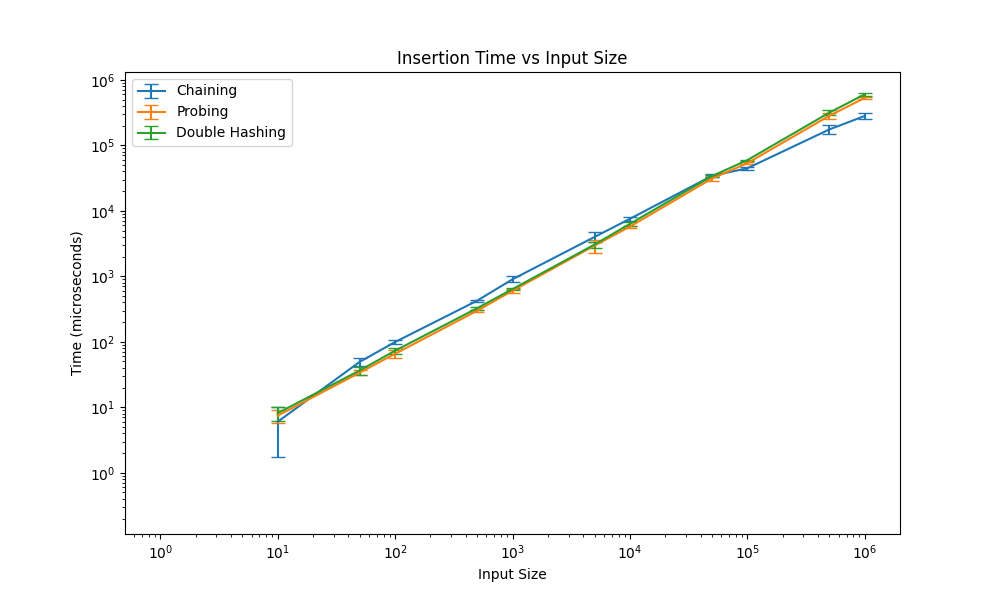
\includegraphics[width=\textwidth]{../plotting/plot_log.png}
    \caption{Time to insert elements vs number of elements to insert with logarithmic scale}
\end{figure}

\begin{figure}[H]
    \centering
    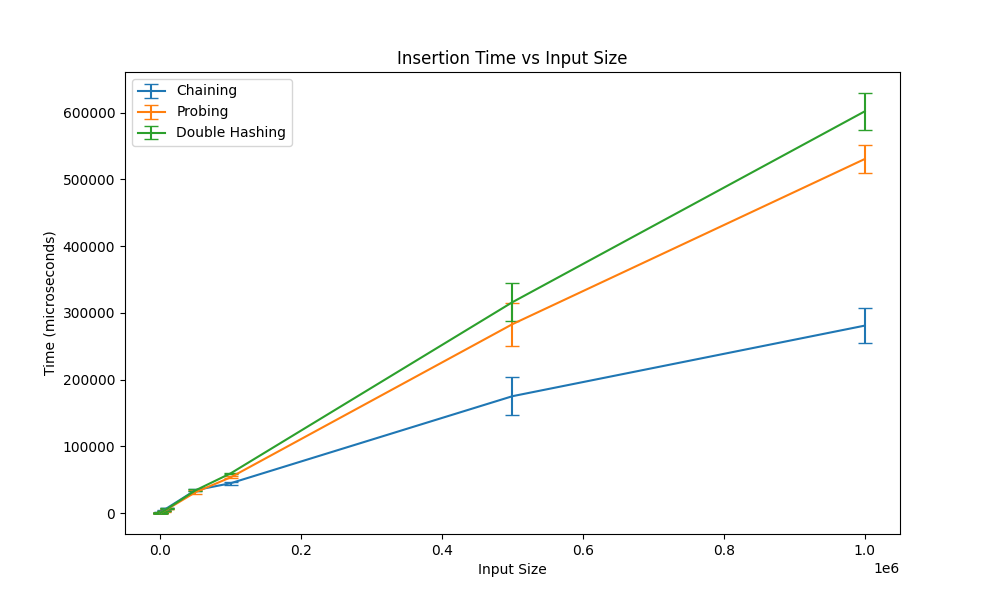
\includegraphics[width=\textwidth]{../plotting/plot_linear.png}
    \caption{Time to insert elements vs number of elements to insert with linear scale}
\end{figure}

\section{Conclusion}
The results gathered from the experiment are quite consistent with the theoretical complexity.
The time to insert elements into the hash table grows approximately linearly with the number of elements to insert, which is expected for a $O(1)$ time complexity, since we have $n$ number of $O(1)$ operations.
If the insert function were not $O(1)$, we would expect to see a much more significant increase in time as the number of elements to insert grows.
In comparison of the three implementations, we can see that separate chaining tends to be the most efficient up to the point where the input size exceeds 50,000 elements.
Past that point, linear probing and double hashing tend to be more efficient.
This is likely due to cache locality, as separate chaining requires the use of linked lists, which are not contiguous in memory, leading to more cache misses.
Across the entire range of input sizes, double hashing tends to be more efficient than linear probing.
This is likely due to the reduced clustering that double hashing provides, which leads to a more even distribution of elements in the hash table, and lessening the need to search for an empty spot in the hash table.
Overall, the experimental results are consistent with the theoretical complexity of the insert function for each of the three implementations.

\end{document}